\chapter{使用GenServer编写服务器应用程序}\label{chapt:genserver}

本章内容包括:

\begin{itemize}

\item  OTP及其使用原因
\item  OTP行为
\item  重写Metex以使用GenServer OTP行为
\item  结构化你的代码以使用GenServer
\item  使用回调处理同步和异步请求
\item  管理服务器状态
\item  干净地停止服务器
\item  为GenServer注册一个名称
\end{itemize}

在本章中,我们首先学习OTP。OTP最初代表Open Telecom Platform。这个名字是由Ericsson的营销天才们创造的(我希望他们不会读到这个!),现在只被称为它的首字母缩写。部分原因是因为这个命名过于短视。OTP提供的工具并不特定于电信领域。然而,这个名字还是被保留下来了,无论好坏。这只是证明了命名确实是计算机科学中最难的问题之一。

我们将学习OTP到底是什么。然后我们将看一下驱动其创建的一些动机。我们还将看到OTP的\emph{行为(Behaviours)}如何帮助我们构建应用程序,减少样板代码,大幅减少潜在的并发错误,并依赖于经过数十年艰苦经验积累的代码。

一旦我们理解了OTP的核心原则,我们将学习一个最重要和最常见的OTP行为 - \texttt{GenServer}。\texttt{GenServer}是Generic Server的简称,\texttt{GenServer}行为是客户端/服务器功能的抽象。我们将把在第3章中构建的温度报告应用程序\texttt{Metex},转变成一个\texttt{GenServer}。到那时,你将对如何实现你自己的\texttt{GenServers}有一个坚实的理解。

 \section{OTP到底是什么?}

OTP有时被称为一个框架,但这并准确。事实上,你应该把OTP看作是一个完整的并发编程开发环境。为了证明我的观点,这里有一个OTP附带功能的非详尽清单:

\begin{itemize}

\item  Erlang解释器和编译器
\item  Erlang标准库
\item  Dialyzer,一个静态分析工具
\item  Mnesia,一个分布式数据库
\item  Erlang Term Storage (ETS),一个内存数据库
\item  一个调试器
\item  一个事件跟踪器
\item  一个发布管理工具
\end{itemize}

我们将在书中的后续部分遇到OTP的各种部分。现在,我们将把注意力转向OTP行为。

 \section{OTP行为}

将OTP行为视为进程的设计模式。这些行为源自经过实战测试的生产代码,并且一直在不断完善。在你的代码中使用OTP行为可以为你提供代码的通用部分,让你只需要实现特定的业务逻辑。

以GenServer为例。GenServer为你提供了开箱即用的客户端/服务器功能。特别是,它提供了所有服务器通用的功能。这些通用功能是什么呢?它们包括:

\begin{itemize}

\item  启动服务器进程
\item  在服务器中维护状态
\item  处理请求并发送回应
\item  停止服务器进程
\end{itemize}

GenServer已经覆盖了通用部分。而你则需要提供业务逻辑。你需要提供的特定逻辑包括:

\begin{itemize}
\item  你想用来初始化服务器的状态
\item  服务器处理的消息类型
\item  何时回复客户端
\item  回复客户端的消息内容
\item  终止后需要清理的资源
\end{itemize}

还有其他的好处。例如,当你正在构建你的服务器应用时,你如何知道你已经覆盖了所有可能出现的必要边缘情况和并发问题呢?此外,理解服务器逻辑的不同实现也不会有趣。

以\texttt{Metex}示例中的\texttt{worker.ex}为例。在我不使用GenServer行为的程序中,我通常将主循环命名为\texttt{loop}。然而,没有人会阻止任何人将其命名为\texttt{await}、\texttt{recur}甚至是像\texttt{while\_1\_true}这样荒谬的名字。使用GenServer行为可以让我(更可能是那些对命名有困难的开发者)免于考虑这些琐事。

\subsection{不同的OTP行为}

下表列出了开箱即用的常见OTP行为。OTP并不限制你只使用这四种。事实上,你可以实现你自己的行为。然而,理解如何正确使用默认的行为是至关重要的,因为它们覆盖了你可能遇到的大多数用例。

\begin{longtable}[]{@{}ll@{}}
\toprule()
行为 & 描述 \\
\midrule()
\endhead
GenServer & 用于实现客户端-服务器关系的服务器的行为模块。 \\
GenEvent & 用于实现事件处理功能的行为模块 \\
Supervisor & 用于实现监督功能的行为模块 \\
Application & 用于处理应用程序和定义应用程序回调的模块。 \\
\bottomrule()
\caption{OTP行为及其提供的功能}
\label{table:otp_behaviours}
\end{longtable}

为了使事情更具体,我们可以亲自看看这些行为是如何组合在一起的。为此,我们需要OTP免费提供的Observer工具。启动\texttt{iex},并启动Observer:

\begin{code}{启动Observer工具}
\begin{minted}[linenos]{elixir}
% iex
iex(1)> :observer.start
:ok
\end{minted}
\label{lst:start_observer}
\end{code}

当窗口弹出时,点击``Applications''选项卡。你应该会看到类似这样的内容:

\begin{figure}[!ht]
    \centering
    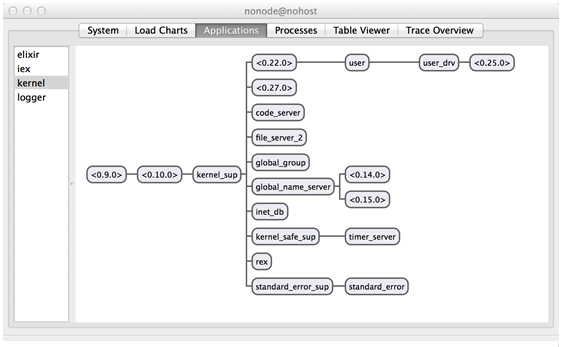
\includegraphics[width=0.8\linewidth]{4_2.png}
    \caption{Observer工具显示Kernel应用的监督器树}
    \label{fig:4_2}
\end{figure}


在左侧列中是一个OTP\emph{应用(Application)}的列表,这些应用在启动iex时已经启动。
我们将在下一章中介绍应用。现在,你可以将它们视为自包含的程序。
点击左列中的每个选项都会显示该应用的\emph{监督器(Supervisor)}层次结构。例如,上图显示了\texttt{kernel}应用的监督器层次结构,这是在\texttt{elixir}应用启动之前就启动的第一个应用。

如果你仔细观察,你会注意到监督器后面都附加了一个\texttt{sup}。例如,\texttt{kernel\_sup}监督了其他十个进程。
这些进程可能是GenServers(例如\texttt{code\_server}和\texttt{file\_server})或者其他的监督器(例如\texttt{kernel\_safe\_sup}和\texttt{standard\_error\_sup})。

像GenServer和GenEvent这样的行为是\emph{工作进程(Worker)} -它们包含了大部分的业务逻辑,并完成了大部分的繁重工作。
随着我们的进展,你将更多地了解它们。
监督器正如它们听起来的那样:它们监督下面的进程,并在发生不好的事情时采取行动。让我们通过从最常用的OTP行为 - GenServer开始,使一切变得更具体。

\section{动手实践OTP:重新审视Metex}

以GenServer为例,我们将实现一个OTP行为。我们将重新实现第\ref{chapt:processes}章中的天气应用\texttt{Metex}。只是这次,我们将使用GenServer行为来实现它。

如果你需要复习一下,\texttt{Metex}会报告给定位置(如城市名称)的摄氏温度。这是通过对第三方天气服务进行HTTP调用来完成的。我们将添加其他的功能,以说明各种GenServer概念,如保持状态和进程注册。例如,我们将跟踪请求的有效位置的频率。

我们将跳过第\ref{chapt:processes}章中讨论的功能部分。换句话说,如果所有这些对你来说都是新的,那么现在将是开始阅读第\ref{chapt:processes}章的最佳时机!
一旦我们完成了应用程序,我们将退一步,比较第\ref{chapt:processes}章和第\ref{chapt:genserver}章的方法。让我们开始吧!

\subsection{创建一个新项目}

像往常一样,创建一个新项目。记住先把你旧版本的\texttt{Metex}放在另一个目录中!

\begin{code}{}
\begin{minted}[linenos]{elixir}
% mix new metex
\end{minted}
% \label{lst:id}
\end{code}

在\texttt{mix.exs}中,填写\texttt{application}和\texttt{deps},如下所示:

\begin{code}{项目设置}
\begin{minted}[linenos]{elixir}
defmodule Metex.Mixfile do
    use Mix.Project

# ...

    def application do
        [applications: [:logger, :httpoison]]
    end

    defp deps do
        [
        {:httpoison, "~> 0.9.0"},
        {:json,      "~> 0.3.0"}
        ]
    end
end
\end{minted}
\label{lst:project_setting_genserver}
\end{code}

然后我们需要获取我们的依赖项。在终端中,使用\texttt{mix deps.get}命令来做到这一点。

\subsection{使Worker符合GenServer}

我们从应用程序的主力,工作进程开始。在\texttt{lib/worker.ex}中,我们首先声明一个新的模块,并指定我们希望使用GenServer行为:

\begin{code}{使用GenServer行为}
\begin{minted}[linenos]{elixir}
defmodule Metex.Worker do
  # 1
  use GenServer
end

# 1 自动定义GenServer所需的所有回调
\end{minted}
\label{lst:use_genserver_behaviour}
\end{code}

只要有\texttt{use GenServer},Elixir就会自动定义GenServer所需的所有回调。这意味着你可以挑选和选择你想要实现的回调。这些回调到底是什么呢?很高兴你问到这个问题。

 \subsection{ 回调}

有六个回调函数会自动为你定义。以下是完整的列表:

\begin{itemize}

\item  \texttt{init(args)}
\item  \texttt{handle\_call(msg, \{from, ref\}, state)}
\item  \texttt{handle\_cast(msg, state)}
\item  \texttt{handle\_info(msg, state)}
\item  \texttt{terminate(reason, state)}
\item  \texttt{code\_change(old\_vsn, state, extra)}
\end{itemize}

在我们进一步讨论之前,有必要提醒自己,我们为什么要费心让工作进程成为一个GenServer,尤其是(如你很快就会看到的)你需要学习各种回调函数和正确的返回值。

使用OTP的最大好处是,当你编写自己的客户端-服务器程序或监督器时,你不必担心的所有事情。例如,你如何编写一个函数来进行异步请求?同步请求呢?GenServer行为为这个确切的用例提供了\texttt{handle\_cast/2}和\texttt{handle\_call/3}。

你的进程必须处理不同类型的消息。随着消息类型的增多,手动编写的进程可能会变得笨重。再次,GenServer的各种\texttt{handle\_*}函数提供了一种整洁的方式来指定你想要处理的不同类型的消息。接收消息只是一半的问题。你还需要一种处理回复的方式。正如预期的那样,回调函数会帮你解决问题,因为它使得访问发送进程的pid变得方便。

现在让我们考虑一下状态管理。每个进程都需要一种初始化状态的方式。它也需要一种在进程终止之前可能进行一些清理的方式。GenServer的\texttt{init/1}和\texttt{terminate/2}就是你需要的回调。

回想一下在上一章中,我们是如何使用递归循环并将(可能)修改过的状态传递给该循环的下一次调用来管理状态的。不同回调的返回值会影响状态。在一个非平凡的进程中手动实现这一点会导致代码看起来很笨拙。

使用GenServer也使得它很容易被插入到比如说,一个监督器中。编写符合OTP行为的程序的好处是,它们看起来往往相似。这意味着,如果你看别人的GenServer,你很可能会很容易地知道它可以处理哪些消息,它可以给出什么回复,以及回复是同步的还是异步的。

现在你知道了只需输入\texttt{use GenServer}就能得到的一些好处。Elixir自动定义了GenServer所需的所有回调。在Erlang中,你需要指定相当多的样板代码。这意味着你可以挑选和选择你想要实现的回调。这些回调到底是什么呢?很高兴你问到这个问题。

\begin{longtable}[]{@{}ll@{}}
\toprule()
GenServer模块调用 & 回调模块(在Metex.Worker中实现) \\
\midrule()
\endhead
\texttt{GenServer.start\_link/3} &
\texttt{Metex.init/1} \\
\texttt{GenServer.call/3} &
\texttt{Metex.handle\_call/3} \\
\texttt{GenServer.cast/2} &
\texttt{Metex.handle\_cast/2} \\
\bottomrule()
\caption{GenServer函数与Metex.Worker的对比}
\label{table:genserver_metex}
\end{longtable}

每个回调都期望一个符合GenServer期望的返回值。下面是一个表格,总结了回调、调用它们的函数以及期望的返回值。当你需要确定每个回调期望的确切返回值时,你会发现这个表格特别有帮助。我发现自己经常参考这个表格。


\begin{longtable}[]{@{}ll@{}}
\toprule()
回调 & 期望的返回值 \\
\midrule()
\endhead
\mintinline{elixir}|init(args)| &
\mintinline{elixir}|{:ok, state}| \\
& \mintinline{elixir}|{:ok, state, timeout}| \\
& \mintinline{elixir}|:ignore| \\
& \mintinline{elixir}|{:stop, reason}| \\
\mintinline{elixir}|handle_call(msg, \{from, ref\},state)| &
\mintinline{elixir}|{:reply, reply, state}| \\
& \mintinline{elixir}|{:reply, reply, state, timeout}| \\
& \mintinline{elixir}|{:reply, reply, state, :hibernate}| \\
& \mintinline{elixir}|{:noreply, state}| \\
& \mintinline{elixir}|{:noreply, state, timeout}| \\
& \mintinline{elixir}|{:noreply, state, hibernate}| \\
& \mintinline{elixir}|{:stop, reason, reply, state}| \\
& \mintinline{elixir}|{:stop, reason, state}| \\
\mintinline{elixir}|handle_cast(msg, state)| &
\mintinline{elixir}|{:noreply, state}| \\
& \mintinline{elixir}|{:noreply, state, timeout}| \\
& \mintinline{elixir}|{:noreply, state, :hibernate}| \\
& \mintinline{elixir}|{:stop, reason, state}| \\
\mintinline{elixir}|handle_info(msg, state)| &
\mintinline{elixir}|{:noreply, state}| \\
& \mintinline{elixir}|{:noreply, state, timeout}| \\
& \mintinline{elixir}|{:stop, reason, state}| \\
\mintinline{elixir}|terminate(reason, state)| &
\mintinline{elixir}|:ok| \\
\mintinline{elixir}|code_change(old_vsn, state, extra)| &
\mintinline{elixir}|{:ok, new_state}| \\
& \mintinline{elixir}|{:error, reason}| \\
\bottomrule()
\caption{GenServer回调及其期望的返回值}
\label{table:genserver_callbacks}
\end{longtable}

当调用\texttt{GenServer.start\_link/3}时,会调用\texttt{init(args)}。让我们在代码中看看:

\begin{code}{用客户端API、服务器回调和辅助函数结构化代码}
\begin{minted}[linenos]{elixir}
defmodule Metex.Worker do
  use GenServer

  ## Client API

  def start_link(opts \\ []) do
    GenServer.start_link(__MODULE__, :ok, opts)
  end

  ## Server Callbacks

  def init(:ok) do
    {:ok, %{}}
  end

  ## Helper Functions
end
\end{minted}
\label{lst:structure_code}
\end{code}

在这里,我通过注释划分了不同的代码部分。你通常会发现野生的Elixir/Erlang程序遵循类似的约定。由于我们还没有引入任何辅助函数,所以``辅助函数''部分被留空。

\subsubsection{\texttt{start\_link/3} 和\texttt{init/1}}

\texttt{GenServer.start\_link/3}接受GenServer实现的模块名,其中定义了\texttt{init/1}回调。它启动进程并将服务器进程链接到父进程。这意味着,如果服务器进程由于某种原因失败,父进程将被通知。

第二个参数是要传递给\texttt{init/1}的参数。由于我们不需要任何参数,所以\texttt{:ok}就足够了。

最后一个参数是要传递给\texttt{GenServer.start\_link/3}的选项列表。这些选项包括定义一个名字来注册进程和启用额外的调试信息。现在,我们可以传入一个空列表。

当调用\texttt{GenServer.start\_link/3}时,它会调用\texttt{Metex.init/1}。它会等待\texttt{Metex.init/1}返回后再返回。\texttt{Metex.init/1}的有效返回值是什么呢?查阅表格,我们得到以下四个值:

\begin{itemize}

\item  \mintinline{elixir}|{:ok, state}|
\item  \mintinline{elixir}|{:ok, state, timeout}|
\item  \texttt{:ignore}
\item  \mintinline{elixir}|{:stop, reason}|
\end{itemize}

现在,我们选择最简单的,\mintinline{elixir}|{:ok state}|。看看我们的实现,这种情况下的\texttt{state}被初始化为一个空的Map,\texttt{\%\{\}}。我们需要这个map来保持请求位置的频率。

让我们试一试!打开你的控制台并启动\texttt{iex}:

\texttt{\% iex -S mix}

现在让我们启动一个服务器进程并将其链接到调用进程。在这种情况下,它是shell进程:

\begin{code}{启动服务器进程}
\begin{minted}[linenos]{elixir}
iex(1)> {:ok, pid} = Metex.Worker.start_link
{:ok, #PID<0.134.0>}
\end{minted}
\label{lst:start_server_process}
\end{code}

结果是一个两元素的元组,和\texttt{:ok}以及新服务器进程的pid。


\subsection{使用 \texttt{handle\_call/3} 处理同步请求}

让我们回到代码。现在,我们希望我们的服务器进程处理请求,这是有服务器进程的全部意义。让我们从客户端API开始,然后向下工作。

\begin{code}{使用 \texttt{GenServer.call/3} 实现同步请求}
\begin{minted}[linenos]{elixir}
defmodule Metex.Worker do
  use GenServer

  ## Client API

  # ...

  def get_temperature(pid, location) do
    GenServer.call(pid, {:location, location})
  end

  ## Server API

  # ...
end
\end{minted}
\label{lst:use_genserver_call}
\end{code}

客户端可能会这样获取新加坡的温度:

\begin{code}{}
\begin{minted}[linenos]{elixir}
Metex.Worker.get_temperature(pid, "Singapore").
\end{minted}
% \label{lst:id}
\end{code}

上述函数包装了对\texttt{GenServer.call/3}的调用,传入pid和一个带有\texttt{:location}标签和实际\texttt{location}的元组。反过来,\texttt{GenServer.call/3}期望在\texttt{Metex.Worker}模块中定义一个\texttt{handle\_call/3}并相应地调用它。

\texttt{GenServer.call/3}向服务器发出\emph{同步}请求。这意味着期望服务器的回复。\texttt{GenServer.call/3}的兄弟是\texttt{GenServer.cast/2},它向服务器发出\emph{异步}请求。我们稍后会看到这个。现在,这是\mintinline{elixir}|{:location, location}|消息的\texttt{handle\_call/3}的实现:


\begin{code}{实现 \texttt{handle\_call} 回调}
\begin{minted}[linenos]{elixir}
defmodule Metex.Worker do
use GenServer

## Client API

# ...

def get_temperature(pid, location) do
GenServer.call(pid, {:location, location})
end

## Server API

# ...

def handle_call(#1{:location, location}, #2_from, #3stats) do
case temperature_of(location) do
{:ok, temp} ->
new_stats = update_stats(stats, location)
{:reply, "#{temp}°C", new_stats}

_ ->
{:reply, :error, stats}
end
end
end

#1: 预期要处理的请求
#2: 这实际上是一个形式为 {pid, tag} 的元组,表示发送者的 pid和消息的唯一引用
#3: GenServer 的当前状态
\end{minted}
\label{lst:use_handle_call}
\end{code}

首先,让我们仔细看一下函数参数:

\begin{code}{}
\begin{minted}[linenos]{elixir}
def handle_call({:location, location}, _from, stats) do
# ...end
\end{minted}
% \label{lst:id}
\end{code}

第一个参数声明了预期要处理的请求。第二个参数返回一个形式为\mintinline{elixir}|{pid, tag}|的元组,其中\texttt{pid}是客户端的pid,\texttt{tag}是消息的唯一引用。第三个参数,\texttt{state},表示服务器的\emph{内部状态}。在我们的情况下,它是当前有效位置的频率计数。

现在,让我们关注\mintinline{elixir}|handle_call({:location, location}, ...)|的主体:

\begin{code}{}
\begin{minted}[linenos]{elixir}
def handle_call({:location, location}, _from, stats) do
    case temperature_of(location) do              #1
        {:ok, temp} ->
            new_stats = update_stats(stats, location) #2
            {:reply, "#{temp}°C", new_stats}          #3

        _ -> {:reply, :error, stats}                   #3
    end
end

#1: 向 API 请求位置的温度 
#2: 使用位置频率更新Map stats  
#3: 返回一个作为响应的三元素元组。
\end{minted}
% \label{lst:id}
\end{code}



\texttt{Metex.Worker.temperature\_of/1}向第三方API发出请求,以获取位置的温度。
如果成功,\texttt{Metex.Worker.update\_stats/2}被调用,返回一个带有更新的位置频率的新Map。
最后,它返回一个任何\texttt{handle\_call/3}都期望返回的三元素元组。

特别是,这个三元组以\texttt{:reply}开始,然后是实际计算的响应,然后是更新的状态,这种情况下是\texttt{new\_stats}。
如果出于某种原因向第三方API的请求失败,那么将返回\mintinline{elixir}|{:reply, :error, stats}|。以下是\texttt{handle\_call/3}的有效响应:

\begin{itemize}

\item  \mintinline{elixir}|{:reply, reply, state}|
\item  \mintinline{elixir}|{:reply, reply, state, timeout}|
\item  \mintinline{elixir}|{:reply, reply, state, :hibernate}|
\item  \mintinline{elixir}|{:noreply, state}|
\item  \mintinline{elixir}|{:noreply, state, timeout}|
\item  \mintinline{elixir}|{:noreply, state, hibernate}|
\item  \mintinline{elixir}|{:stop, reason, reply, state}|
\item  \mintinline{elixir}|{:stop, reason, state}|
\end{itemize}

让我们填补一下缺失的部分,以便让\texttt{Metex.Worker.get\_temperature/2}工作:

\begin{code}{实现辅助函数}
\begin{minted}[linenos]{elixir}
defmodule Metex.Worker do
  use GenServer

  ## Client API and Server API

  ## previously implemented code

  ## Helper Functions

  defp temperature_of(location) do
    url_for(location) |> HTTPoison.get() |> parse_response
  end

  defp url_for(location) do
    "http://api.openweathermap.org/data/2.5/weather?q=#{location}&APPID=#{apikey}"
  end

  defp parse_response({:ok, %HTTPoison.Response{body: body, status_code: 200}}) do
    body |> JSON.decode!() |> compute_temperature
  end

  defp parse_response(_) do
    :error
  end

  defp compute_temperature(json) do
    try do
      temp = (json["main"]["temp"] - 273.15) |> Float.round(1)
      {:ok, temp}
    rescue
      _ -> :error
    end
  end

  def apikey do
    "APIKEY-GOES-HERE"
  end

  defp update_stats(old_stats, location) do
    case Map.has_key?(old_stats, location) do
      true ->
        Map.update!(old_stats, location, &(&1 + 1))

      false ->
        Map.put_new(old_stats, location, 1)
    end
  end
end
\end{minted}
\label{lst:helper_functions}
\end{code}

大部分的实现与第\ref{chapt:processes}章相同,只是对\texttt{Metex.Worker.temperature\_of/1}和\texttt{Metex.Worker.update\_stats/2}做了一些小的修改,这两个函数是全新的。
\texttt{Metex.Worker.update\_stats/2}的实现非常简单:

\begin{code}{更新请求位置的频率}
\begin{minted}[linenos]{elixir}
defp update_stats(old_stats, location) do
  case Map.has_key?(old_stats, location) do
    true ->
      Map.update!(old_stats, location, &(&1 + 1))

    false ->
      Map.put_new(old_stats, location, 1)
  end
end
\end{minted}
\label{lst:update_stats}
\end{code}

这个函数接收\texttt{old\_stats}和请求的\texttt{location}。我们首先检查\texttt{old\_stats}是否包含位置的键。如果是,我们可以简单地获取值并增加计数器。否则,我们放入一个由\texttt{location}表示的新键,并将其设置为\texttt{1}。如果\texttt{\&(\&1 + 1)}的匿名函数写法看起来让人困惑,你可以在你的脑海中进行语法``去糖化'':

\begin{code}{}
\begin{minted}[linenos]{elixir}
Map.update!(old_stats, location, fn val -> val + 1 end)
\end{minted}
% \label{lst:id}
\end{code}

让我们再次尝试一下\texttt{Metex.Worker}。再次启动\texttt{iex},然后使用\texttt{Metex.Worker.start\_link/1}启动服务器:

\begin{code}{}
\begin{minted}[linenos]{elixir}
% iex -S mix
iex(1)> {:ok, pid} = Metex.Worker.start_link
{:ok, #PID<0.125.0>}
\end{minted}
% \label{lst:id}
\end{code}

现在,让我们从一些著名的地点获取温度:

\begin{code}{}
\begin{minted}[linenos]{elixir}
iex(2) > Metex.Worker.get_temperature(pid, "Babylon")
"12.7°C"
iex(3) > Metex.Worker.get_temperature(pid, "Amarillo")
"5.3°C"
iex(4) > Metex.Worker.get_temperature(pid, "Memphis")
"7.3°C"
iex(5) > Metex.Worker.get_temperature(pid, "Rio")
"23.5°C"
iex(6) > Metex.Worker.get_temperature(pid, "Philadelphia")
"12.5°C"
\end{minted}
% \label{lst:id}
\end{code}


\subsection{访问服务器状态}

成功了!但等一下,我如何查看\texttt{stat}的内容呢?换句话说,我们如何访问\emph{服务器状态}?事实证明,这并不难。让我们首先实现面向客户端的API:

\begin{code}{}
\begin{minted}[linenos]{elixir}
def get_stats(pid) do
  GenServer.call(pid, :get_stats)
end
\end{minted}
% \label{lst:id}
\end{code}

由于我们期望服务器的回复,我们需要服务器的同步回复。因此,我们应该调用\texttt{GenServer.call/3}。在这里,我们说服务器应该处理一个同步的\texttt{:get\_stats}消息。注意,消息可以是任何有效的Elixir项的形式。这意味着元组、列表和原子都是合法的返回值。这是回调函数:

\begin{code}{}
\begin{minted}[linenos]{elixir}
def handle_call(:get_stats, _from, stats) do
  {:reply, stats, stats}
end
\end{minted}
% \label{lst:id}
\end{code}

由于我们对\texttt{stats}感兴趣,我们可以在第二个参数中简单地返回\texttt{stats}作为回复。由于我们只是访问\texttt{stats},而不是修改它,我们简单地将其保持不变作为第三个参数。

在我们继续之前,这里有一个温馨的提醒,要\emph{将所有的\texttt{handle\_call}(以及稍后的\texttt{handle\_cast})分组在一起}!这很重要,因为Erlang虚拟机依赖于这个进行模式匹配。例如,如果我''误放''了\texttt{handle\_call},就像这样:

\begin{code}{注意 \texttt{handle\_calls} 没有分组在一起}
\begin{minted}[linenos]{elixir}
defmodule Metex.Worker do
  use GenServer

  ## Client API

  # ...

  ## Server Callbacks

  # 1
  def handle_call(:get_stats, _from, stats) do
    # ...
  end

  def init(:ok) do
    # ...
  end

  def handle_call({:location, location}, _from, stats) do
    # ...
  end

  ## Helper Functions

  # ...
end

# 1: handle_calls 和 handle_casts 应该分组在一起
\end{minted}
\label{lst:note_handle_calls}
\end{code}

然后,编译器会发出一个友好的警告:

\begin{code}{}
\begin{minted}[linenos]{elixir}
% iex -S mix
lib/worker.ex:29: warning: clauses for the same def should be grouped together, def handle_call/3 was previously defined (lib/worker.ex:20)
\end{minted}
% \label{lst:id}
\end{code}


\subsection{使用 \texttt{handle\_cast/2} 处理异步请求}

异步请求不需要服务器的回复。这也意味着\texttt{GenServer.cast/2}会立即返回。对于\texttt{GenServer.cast/2}来说,什么是一个好的用例呢?一个很好的例子是向服务器发出一个命令,这个命令会在服务器的状态中产生一些副作用。在这种情况下,发出命令的客户端不应该关心回复。

让我们构造这样一个命令。这个命令叫做\texttt{reset\_stats},它将把stats重新初始化为一个空的Map:

\begin{code}{处理重置统计}
\begin{minted}[linenos]{elixir}
# Client API

# ...

def reset_stats(pid) do
  GenServer.cast(pid, :reset_stats)
end

# Server Callbacks

# handle_calls go here

def handle_cast(:reset_stats, _stats) do
  {:noreply, %{}}
end
\end{minted}
\label{lst:hangle_reset_stats}
\end{code}

\texttt{Metex.Worker.stats/1}将调用\texttt{GenServer.cast/2}。这反过来又调用了\texttt{handle\_cast(:reset\_stats, \_stats)}回调。由于我们不关心服务器的当前状态(毕竟,我们正在重置它),我们在\texttt{stats}前面加上一个下划线。

返回值是一个两元素的元组,第一个元素是\texttt{:noreply},第二个元素是一个空的Map,也就是响应。再次注意,响应是有效的\texttt{handle\_cast/2}响应之一。

让我们看看我们的成果!再次启动\texttt{iex -S mix},然后尝试一些位置:

\begin{code}{}
\begin{minted}[linenos]{elixir}
iex(1)> {:ok, pid} = Metex.Worker.start_link
{:ok, #PID<0.134.0>}
iex(2)> Metex.Worker.get_temperature pid, "Singapore"
"29.0°C"
iex(3)> Metex.Worker.get_temperature pid, "Malaysia"
"22.7°C"
iex(4)> Metex.Worker.get_temperature pid, "Brunei"
"24.2°C"
iex(5)> Metex.Worker.get_temperature pid, "Singapore"
"29.0°C"
iex(6)> Metex.Worker.get_temperature pid, "Cambodia"
"27.7°C"
iex(7)> Metex.Worker.get_temperature pid, "Brunei"
"24.2°C"
iex(8)> Metex.Worker.get_temperature pid, "Singapore"
"29.0°C"
\end{minted}
% \label{lst:id}
\end{code}

现在我们可以尝试一下 \texttt{get\_stats/1} 函数:

\begin{code}{}
\begin{minted}[linenos]{elixir}
iex(9) > Metex.Worker.get_stats(pid)
%{"Brunei" => 2, "Cambodia" => 1, "Malaysia" => 1, "Singapore" => 3}
\end{minted}
% \label{lst:id}
\end{code}

它工作了!你可以清楚地看到由Map表示的请求位置的频率。现在,让我们试着重置\texttt{stats}:

\begin{code}{}
\begin{minted}[linenos]{elixir}
iex(10) > Metex.Worker.reset_stats(pid)
:ok
iex(11) > Metex.Worker.get_stats(pid)
%{}
\end{minted}
% \label{lst:id}
\end{code}

完美!它按预期工作了。


\subsection{停止服务器并清理}

有时,我们需要在服务器停止之前释放资源,或者进行一些其他的清理任务。这就是\texttt{GenServer.terminate/2}的作用。

那么我们如何停止服务器呢?如果你查看回调表,在\texttt{handle\_call/handle\_cast}列下,你会发现两个以\texttt{:stop}开头的有效响应:

\begin{itemize}
\item  \mintinline{elixir}|{:stop, reason, new_state}|
\item  \mintinline{elixir}|{:stop, reason, reply, new_state}|
\end{itemize}

这是一个信号,告诉GenServer服务器将被终止。因此,我们需要做的就是提供一个返回上述响应的任意一个的回调(来自\texttt{handle\_call/3}或\texttt{handle\_cast/2}),并在\texttt{GenServer.terminate/2}回调中包含清理逻辑。我们首先在客户端API下写一个\texttt{stop/1}函数:

\begin{code}{}
\begin{minted}[linenos]{elixir}
def stop(pid) do
  GenServer.cast(pid, :stop)
end
\end{minted}
% \label{lst:id}
\end{code}

再次,我选择了\texttt{GenServer.cast/2},因为我并不真正关心任何返回值。另一个原因可能是服务器可能需要时间来正确地清理所有资源,而我不想等待。相应的回调非常简单:

\begin{code}{}
\begin{minted}[linenos]{elixir}
def handle_cast(:stop, stats) do
  {:stop, :normal, stats}
end
\end{minted}
% \label{lst:id}
\end{code}

我们没有任何资源可以说的,但你可以想象我们可能会例如将\texttt{stats}写入文件或数据库。在我们的例子中,让我们在停止服务器之前打印当前状态:

\begin{code}{终止回调在服务器终止之前被调用}
\begin{minted}[linenos]{elixir}
def terminate(reason, stats) do
  # 我们可以写入文件、数据库等
  IO.puts("server terminated because of #{inspect(reason)}")
  inspect(stats)
  :ok
end
\end{minted}
\label{lst:stop_callback_before_server_terminates}
\end{code}

\texttt{GenServer.terminate/2}有两个参数。第一个参数提供了服务器终止的原因。在正常终止时,原因将是\texttt{:normal}。\texttt{:normal}来自早期定义的\texttt{handle\_cast/2}的响应。对于错误,例如由于捕获到的异常,你可以包含其他原因。最后,\texttt{GenServer.terminate/2}必须始终返回\texttt{:ok}。让我们看看我们如何在iex中终止一个服务器。

\begin{code}{}
\begin{minted}[linenos]{elixir}
% iex -S mix
iex(1)> {:ok, pid} = Metex.Worker.start_link
{:ok, #PID<0.152.0>}
iex(2)> Process.alive? pid
true
iex(3)> Metex.Worker.stop pid
server terminated because of :normal
:ok
iex(4)> Process.alive? pid
false
\end{minted}
% \label{lst:id}
\end{code}


\subsection{当回调返回无效响应时会发生什么?}

让我们稍微修改一下\texttt{handle\_cast(:stop, stats)}的返回值:

\begin{code}{}
\begin{minted}[linenos]{elixir}
def handle_cast(:stop, stats) do
  {:stop, :normal, :ok, stats}
end
\end{minted}
% \label{lst:id}
\end{code}

如果你再看一下表格,这对应于一个有效的\texttt{handle\_call/3}响应,而不是\texttt{handle\_cast/2}!多余的\texttt{:ok}是为了回复客户端。由于\texttt{handle\_cast/2}并不是为了回复客户端(至少,不是直接回复),所以这显然是错误的。让我们看看当我们重复停止服务器的过程时会发生什么:


\begin{code}{当回调没有返回预期的响应时,GenServer会报错}
\begin{minted}[linenos]{elixir}
% iex -S mix
iex(1)> {:ok, pid} = Metex.Worker.start_link
{:ok, #PID<0.152.0>}
iex(2)> Metex.Worker.stop pid
iex(2)>
10:59:15.906 [error] GenServer #PID<0.134.0> terminating #1
Last message: {:"$gen_cast", :stop}                      #1
State: %{}                                               #1
** (exit) bad return value: {:stop, :normal, :ok, %{}}   #1
#1 GenServer在收到回调处理器的无效响应时报告错误
\end{minted}
\label{lst:invalid_response}
\end{code}

首先,注意到这里\emph{没有}编译时错误。只有当我们试图停止服务器时,错误才会浮出水面,GenServer会抛出一个
\mintinline{elixir}|{bad return value: {:stop, :normal, :ok, %{}}}|。
每当你看到这样的东西,你的第一反应应该是仔细检查你的回调处理器的返回值。有时候很容易忽略一些小细节,而且错误信息一开始可能并不那么明显。


\subsection{接收其他类型的消息}

可能会有来自其他进程的消息,这些消息可能没有在\texttt{handle\_call/3}/\texttt{handle\_cast/2}中定义。这就是\texttt{handle\_info/2}的作用。它被调用来处理进程接收到的任何其他消息,有时被称为``带外''消息。你不需要为\texttt{handle\_info/2}提供一个客户端API对应项。这个回调接收两个参数,接收到的消息和当前的状态:

\begin{code}{}
\begin{minted}[linenos]{elixir}
def handle_info(msg, stats) do
  IO.puts("received #{inspect(msg)}")
  {:noreply, stats}
end
\end{minted}
% \label{lst:id}
\end{code}

让我们看看这个在实践中的应用:


\begin{code}{有了 \texttt{handle\_info},服务器进程可以处理任何类型的意外消息}
\begin{minted}[linenos]{elixir}
iex(1)> {:ok, pid} = Metex.Worker.start_link
{:ok, #PID<0.134.0>}
iex(2)> send pid, "It's raining men"
received "It's raining men"
\end{minted}
\label{lst:handle_info_can_handle_any_type_of_message}
\end{code}

我们将在后面的章节中看到更多有趣的\texttt{handle\_info/2}的用途。主要要记住的是,\texttt{handle\_info/2}用于处理任何其他不被\texttt{handle\_call/3}/\texttt{handle\_cast/2}覆盖的消息。

 \subsection{进程注册}

不断通过pid引用GenServer可能会很痛苦。幸运的是,还有另一种方法可以做到这一点。\texttt{GenServer.start\_link/3}接受一个选项列表作为它的第三个参数。

有两种常见的方式可以用一个名字注册一个GenServer,区别在于名字应该在本地还是全局可见。
如果名字被全局注册,那么名字在连接的节点集群(你将很快了解到分布式集群)中是唯一的。
另一方面,本地注册的名字只在本地节点内可见。

对于单例GenServer来说,有一个注册的名字是很好的。也就是说,只应该在一个节点或集群中存在一个。我们将让\texttt{Metex.Worker}在\texttt{MW}下注册。当我们选择为GenServer注册一个名字时,我们就不再需要使用它的pid来引用进程。幸运的是,我们只需要改变客户端API中对\texttt{GenServer.call/3}和\texttt{GenServer.cast/2}的调用:

\begin{code}{有了一个明确的名字,就不再需要将pid传递给客户端API}
\begin{minted}[linenos]{elixir}
defmodule Metex.Worker do
  use GenServer

  # 1
  @name MW

  ## Client API

  def start_link(opts \\ []) do
    # 2
    GenServer.start_link(__MODULE__, :ok, opts ++ [name: MW])
  end

  def get_temperature(location) do
    # 3
    GenServer.call(@name, {:location, location})
  end

  def get_stats do
    # 3
    GenServer.call(@name, :get_stats)
  end

  def reset_stats do
    # 3
    GenServer.cast(@name, :reset_stats)
  end

  def stop do
    # 3
    GenServer.cast(@name, :stop)
  end

  # The rest of the code remains unchanged.
  # ...
end

# 1 存储名字
# 2 用一个注册的名字初始化服务器
# 3 注意我们传递的是 @name 而不是 pid
\end{minted}
\label{lst:with_a_named_server_we_no_longer_need_to_pass_pids_to_the_client_api}
\end{code}


现在,再次启动\texttt{iex -S mix}。这次,我们不需要显式地捕获pid。然而,这是一个好主意,因为我们通常想知道服务器是否正确启动,因此我们希望确保匹配到\texttt{:ok}。

现在,我们可以这样与\texttt{Metex.Worker}交互:

\begin{code}{}
\begin{minted}[linenos]{elixir}
% iex -S mix
iex(1)> Metex.Worker.start_link
{:ok, #PID<0.134.0>}
iex(2)> Metex.Worker.get_temperature "Singapore"
"29.3°C"
iex(3)> Metex.Worker.get_temperature "London"
"2.0°C"
iex(4)> Metex.Worker.get_temperature "Hong Kong"
"24.0°C"
iex(5)> Metex.Worker.get_temperature "Singapore"
"29.3°C"
iex(6)> Metex.Worker.get_stats
%{"Hong Kong" => 1, "London" => 1, "Singapore" => 2}
iex(7)> Metex.Worker.stop
server terminated because of :normal
:ok
\end{minted}
% \label{lst:id}
\end{code}


\subsection{回顾第3章的Metex}

再看一下我们在第\ref{chapt:processes}章中构建的\texttt{Metex}。试着想象一下我们需要添加什么才能获得与本章中构建的\texttt{Metex}相同的功能。另外,试着想象一下你会把所有这些功能放在哪里。

你可能会意识到,有些功能并不容易实现。例如,你如何实现同步和异步调用?停止服务器呢?在这种情况下,我们必须特别处理停止消息,而不是运行循环。那么我们应该在哪里放置清理资源的逻辑呢?

在早期版本的\texttt{Metex.Worker}中,我们必须在循环中使用通配符操作符(即下划线)显式处理意外消息。在OTP中,这是通过\texttt{handle\_info/2}回调处理的。服务器的停止也没有被处理。

考虑到所有这些问题,你很快就会意识到循环函数的大小会开始膨胀。当然,你总是可以把所有的东西抽象出来,放在漂亮的小函数中,但这只能做到一定程度。

希望你能开始看到OTP的好处。使用OTP行为可以帮助你在代码中获得一致的结构。它使你能够轻松地看到客户端API在哪里,服务器回调是如何定义的,以及辅助方法在哪里。

除了提供一致性,OTP还提供了许多对所有类似服务器的程序都有用的功能。例如,使用GenServer管理状态非常简单。你不再需要将你的状态放在一个循环中。能够在回调中决定何时改变你的状态也非常有用。

 \section{练习}

编写一个GenServer,可以存储任何有效的Elixir项,给定一个键。以下是一些可以让你开始的操作:

\begin{itemize}
\item  \texttt{Cache.write(:stooges, ["Larry", "Curly", "Moe"])}
\item  \texttt{Cache.read(:stooges)}
\item  \texttt{Cache.delete(:stooges)}
\item  \texttt{Cache.clear}
\item  \texttt{Cache.exist?(:stooges)}
\end{itemize}

按照我们在本章中的方式来构造你的程序。特别注意上述哪些操作应该是\texttt{handle\_call}或\texttt{handle\_cast}。

\section{总结}

当我第一次学习GenServer时,我需要接受很多信息------这还是轻描淡写的说法。下面的表格可以帮助你将所有相关的函数分组在一起。

我缩写了一些函数名,将\texttt{Metex.Worker}缩写为\texttt{MW},将\texttt{GenServer}缩写为\texttt{GS}。\texttt{state}被缩短为\texttt{st},\texttt{from}被缩短为\texttt{fr}。最后,\texttt{pid}是\texttt{p}。


\begin{longtable}[]{@{}
  >{\raggedright\arraybackslash}p{(\columnwidth - 4\tabcolsep) * \real{0.3333}}
  >{\raggedright\arraybackslash}p{(\columnwidth - 4\tabcolsep) * \real{0.3333}}
  >{\raggedright\arraybackslash}p{(\columnwidth - 4\tabcolsep) * \real{0.3333}}@{}}
\toprule()
\begin{minipage}[b]{\linewidth}\raggedright
Metex.Worker 客户端API
\end{minipage} & \begin{minipage}[b]{\linewidth}\raggedright
GenServer
\end{minipage} & \begin{minipage}[b]{\linewidth}\raggedright
Metex.Worker 回调
\end{minipage} \\
\midrule()
\endhead
\mintinline{elixir}|MW.start_link(:ok)| &
\mintinline{elixir}|GS.start_link| &
\mintinline{elixir}|MW.init(:ok)| \\
\mintinline{elixir}|MW.get_temp(p,"NY")| &
\mintinline{elixir}|GS.call(p,{:loc,"NY"})| &
\mintinline{elixir}|MW.handle_call({:loc, "NY"}, fr, st)| \\
\mintinline{elixir}|MW.reset(p)| &
\mintinline{elixir}|GS.cast(p, :reset)| &
\mintinline{elixir}|MW.handle_cast(:reset, st)| \\
\mintinline{elixir}|MW.stop(p)| &
\mintinline{elixir}|GS.cast(p, :stop)| &
\mintinline{elixir}|MW.handle_cast(:stop, st)| \\
& & 如果上述返回\mintinline{elixir}|{:stop, :normal, st}| \\
& & 那么 \\
& & \mintinline{elixir}|MW.terminate(:normal, st)| 将被调用 \\
\bottomrule()
\caption{客户端API、GenServer和回调函数之间关系的总结}
\label{table:summary_of_the_relationship_between_the_client_api_genserver_and_the_callbacks}
\end{longtable}

让我们看一下最后一行。假设我想停止工作进程,我调用\texttt{Metex.Worker.stop/1}。这将反过来调用\texttt{GenServer.cast/2},传入\texttt{pid}和\texttt{:stop}作为参数。触发的回调将是\texttt{Metex.Worker.handle\_cast(:stop, state)}。如果回调返回一个形如\mintinline{elixir}|{:stop, :normal, state}|的元组,那么就会调用\texttt{Metex.Worker.terminate/2}。

在本章中,我们涵盖了很多内容。以下是一些重点:

\begin{itemize}

\item  OTP是什么,以及其背后的原则和动机
\item  可用的不同类型的OTP行为
\item  将Metex转换为使用GenServer
\item  GenServer提供的各种回调
\item  在GenServer中管理状态
\item  按照约定结构化你的代码
\item  进程注册
\end{itemize}

还有一个好处,我一直故意没有告诉你。使用GenServer行为可以让你将GenServers放入一个监督树中。如果你的GenServer崩溃了会发生什么?它将如何影响你系统的其他部分,你如何确保你的系统保持功能?

请继续阅读,亲爱的读者,因为接下来是监督器------这恰好是我最喜欢的OTP特性之一!
